
\documentclass[xcolor={usenames,dvipsnames},12pt,presentation,aspectratio=169]{beamer}

\usepackage[utf8]{inputenc}
\usepackage[brazilian]{babel}
\usepackage{verbatim}
\usepackage{graphicx}
\usepackage{xspace}
\usepackage{amsthm}
\usepackage{url}
\usepackage{array}
\usepackage{hyperref}
\usepackage{times,mathptmx}
\usepackage{pdfpages}
\usepackage{mdframed}
\usepackage{tikz}
\usepackage{alltt}
%\usepackage[usenames,dvipsnames]{xcolor}
%\usepackage[usenames,dvipsnames]{color}
%\usepackage{color}

\usetikzlibrary{arrows,shapes}

\usetheme{Madrid}
%\usetheme{Boadilla}
%\usetheme{Darmstadt}
%\usetheme{Frankfurt}
%\usetheme{CambridgeUS}
%\usetheme{AnnArbor}
%\usecolortheme{beaver}
%\usecolortheme{seahorse}
%\usecolortheme{seagull}
\usecolortheme[named=BrickRed]{structure}

\setbeamercovered{transparent}

\setbeamertemplate{footline}[frame number]
%\setbeamertemplate{navigation symbols}{}
%\setbeamersize{text margin left=1em,text margin right=1em}

\newcommand{\titulo}{Modelos de Programação Paralela}
\newcommand{\disciplina}{ELC139 - Programação Paralela}
\newcommand{\nome}{João Vicente Ferreira Lima (UFSM)}

\lecture[1]{\aula}{aula01}
\def\lecturename{\aula}

\newcommand{\Red}[1]{{\color{red}#1}}
\newcommand{\red}[1]{{\color{red}#1}}
\newcommand{\Blue}[1]{{\color{blue}#1}}
\newcommand{\blue}[1]{{\color{blue}#1}}

\newcommand{\PBS}[1]{\let\temp=\\#1\let\\=\temp}
\newcommand{\RRCOL}{\PBS\raggedright\hspace{0pt}}

\newcommand{\p}[1]{\texttt{#1}}
\newenvironment{code}{%
  \begin{alltt}%
  }{%
  \end{alltt}%
}

\makeatletter
%\setbeamertemplate{headline}{}
% {%
%   \leavevmode%
%   \@tempdimb=2.4375ex%
%   \ifnum\beamer@subsectionmax<\beamer@sectionmax%
%     \multiply\@tempdimb by 4%
%   \else%
%     \multiply\@tempdimb by\beamer@subsectionmax%
%   \fi%
%   \ifdim\@tempdimb>0pt%
%     \advance\@tempdimb by 1.125ex%
%     \begin{beamercolorbox}[wd=.5\paperwidth,ht=\@tempdimb]{section in head/foot}%
%       \vbox to\@tempdimb{\vfil\insertsectionnavigation{.5\paperwidth}\vfil}%
%     \end{beamercolorbox}%
%     \begin{beamercolorbox}[wd=.45\paperwidth,ht=\@tempdimb]{subsection in head/foot}%
%       \vbox
%       to\@tempdimb{\vfil\insertsubsectionnavigation{.45\paperwidth}\vfil}%
%     \end{beamercolorbox}%
%     \begin{beamercolorbox}[wd=.05\paperwidth,ht=\@tempdimb]{subsection in head/foot}%
%       \vbox
%       to\@tempdimb{\vfil\hfil\insertframenumber\vfil\vfil}%
%     \end{beamercolorbox}%
%   \fi%
% }

\def\dohead{\beamer@headcounter=4\relax\beamer@headcounter=1\loop\ifnum\beamer@headcounter<\beamer@totalheads%
  \advance\beamer@headcounter by1\relax%
  \csname @@head\the\beamer@headcounter\endcsname\repeat}

\makeatother

\title[\titulo]{\titulo}

\subtitle{\disciplina}

\author[João V. F. Lima]{\nome}

%\institute[UFSM]{Departamento de Linguagens e Sistemas de Computação \\ Universidade Federal de Santa Maria \\ \url{jvlima@inf.ufsm.br} \\ \url{http://www.inf.ufsm.br/~jvlima}}
\institute[UFSM]{Universidade Federal de Santa Maria \\ \url{jvlima@inf.ufsm.br} \\ \url{http://www.inf.ufsm.br/~jvlima}}
\date{2023/1}

\graphicspath{{.}{figs/}}

\logo{ 
\includegraphics[height=1.5cm,width=1.5cm,keepaspectratio]{logo_inf}    
        
\includegraphics[height=1.5cm,width=1.5cm,keepaspectratio]{logo_ufsm} }

%\titlegraphic{
%	
\includegraphics[width=2cm]{logo_ufsm}
%  \hspace{1cm}
%	
\includegraphics[width=2cm]{logo_inf}
%}

\newtheorem{mydef}{Definição}[section]
%\newtheorem{myteo}{Teorema}[section]
%------------------------------------------------------------------------------
%\newcommand{\xkaapi}{XKaapi\xspace}
%------------------------------------------------------------------------------
% Typesetting Listings
\usepackage{listings}
\lstset{
  language=C++,
  %basicstyle=\scriptsize\ttfamily,
  %basicstyle=\normalsize\ttfamily,
  basicstyle=\small\ttfamily,
  %basicstyle=\footnotesize\ttfamily,
  aboveskip=0pt,
  belowskip=0pt,
  mathescape=false,
  columns=flexible,
  numbers=none,
%  numbers=left,
%  showtabs=true,
%  showspaces=true,
  breaklines=true
}
%------------------------------------------------------------------------------
\lstset{commentstyle=\color{blue}}
%\lstset{stringstyle=\ttfamily}
%\lstset{ classoffset=1, 
%            morekeywords={kaapi,omp,task,data,alloca, declare, reduction, identity, parallel,sync,taskwait,cilk,spawn,tbb,css,cilk\_spawn,cilk\_sync,cilk\_for,offload},
%            keywordstyle=\color{Red}\bfseries
%           }
%\lstset{ classoffset=2, 
%            morekeywords={value,read,write,readwrite,reduction,untied,firstprivate,TaskBodyCPU,TaskBodyGPU,ka,Signature,RW,CW,range2d\_r,range2d\_rw,range2d,Spawn,Fork,Shared\_w,Shared\_r,Shared,a1,target,device,copyin,copyout,input,implements,copy\_deps,RPWP,range2d\_rpwp,rangeindex,Memory,Register,SetStaticSched,Sync,Unregister,Community,System,join\_community,SpawnMain,leave,initialize,terminate,logfile,array,SetArch,ArchHost,ArchCUDA,W,R,gpuStream,pointer\_w,pointer\_r,pointer\_cw,pointer},
%            keywordstyle=\color{Blue}\bfseries
%           }
%\lstset{ classoffset=3, 
%            morekeywords={storage,ld},
%            keywordstyle=\bfseries
%           }
%\lstset{ classoffset=4, 
%            morekeywords={in,out,inout,cout,concurrent},
%            keywordstyle=\color{Red}\bfseries
%           }
%           
\lstset{classoffset=0, showstringspaces=false}
%------------------------------------------------------------------------------
\mdfsetup{
  backgroundcolor=gray!10,
%  roundcorner=10pt,
}
%------------------------------------------------------------------------------
\newcommand{\restorefootline}{\setbeamertemplate{navigation symbols}{}}
%\newcommand{\setfootline}[1]{\setbeamertemplate{navigation symbols}{\textcolor{black}{\textbf{#1}}}}
\newcommand{\includeslides}[4]{%
%  \setfootline{#1}%
  {
    \setbeamercolor{background canvas}{bg=}
    \includepdf[pages={#1},%
    pagecommand={},
%    pagecommand={\begin{frame}[default]{}\end{frame}},
%    #4,%
    turn=false,noautoscale=false,column=false,columnstrict=false,openright=false,frame=false]{#2}%
  }
  %\restorefootline%
}
%------------------------------------------------------------------------------
\begin{document}

\begin{frame}
%  \titlepage
  \maketitle
%  \mode<presentation>
%  {
%    \begin{columns}
%      \begin{column}{0.5\textwidth}
%      \raggedleft
%	
\includegraphics[width=2cm]{logo_ufsm}
%      \end{column}
%      \begin{column}{0.5\textwidth}
%	
\includegraphics[width=2cm]{logo_inf}
%      \end{column}
%    \end{columns}
%  }
\end{frame}

\begin{frame}
    \frametitle{Outline}
    \tableofcontents[hideallsubsections]
%    \tableofcontents
\end{frame}

\AtBeginSection{
  \begin{frame}
    \frametitle{Outline}
    \tableofcontents[currentsection,hideothersubsections]
  \end{frame}
}

%%%%%%%%%%%%%%%%%%%%%%%%%%%%%%%%%%%%%%%%%%%%%%%%%%%%%%%%%%%%%%%%%%%%%%%%%%%%%%
%\section{Introdução}
%%%%%%%%%%%%%%%%%%%%%%%%%%%%%%%%%%%%%%%%%%%%%%%%%%%%%%%%%%%%%%%%%%%%%%%%%%%%%%%
%------------------------------------------------------------------------------
%\begin{frame}
%  \frametitle{Computação Paralela}
%    \begin{itemize}
%        \item Por que Computação Paralela?
%        \item Onde o paralelismo é aplicado?
%        \item Primeiro grande motivador: hardware
%            \begin{itemize}
%                \item Processadores multicore onipresentes
%                \item Limites de chip
%            \end{itemize}
%        \item Segundo: software
%            \begin{itemize}
%                \item Computação Científica
%                \item Data centers e computação em nuvem
%            \end{itemize}
%    \end{itemize}
%\end{frame}
%%%%%%%%%%%%%%%%%%%%%%%%%%%%%%%%%%%%%%%%%%%%%%%%%%%%%%%%%%%%%%%%%%%%%%%%%%%%%%
\section{Programação Paralela}
%%%%%%%%%%%%%%%%%%%%%%%%%%%%%%%%%%%%%%%%%%%%%%%%%%%%%%%%%%%%%%%%%%%%%%%%%%%%%%%
%------------------------------------------------------------------------------
\begin{frame}
  \frametitle{Programação Serial}
  \vspace{-4mm}
  \begin{itemize}
    \item Problema quebrado em uma série de instruções discretas
    \item Instruções são executadas sequencialmente uma depois da outra
    \item Execução em processador único
  \end{itemize}
  \begin{center}
	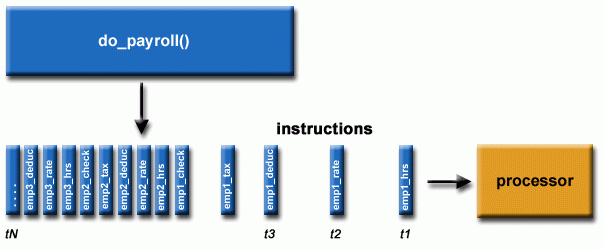
\includegraphics[width=0.5\textwidth]{serialProblem2.png}
  \end{center}
  \vfill
  {\tiny https://hpc.llnl.gov/documentation/tutorials/introduction-parallel-computing-tutorial}
\end{frame}
%------------------------------------------------------------------------------
\begin{frame}
  \frametitle{Programação Paralela}
  \vspace{-2mm}
  \begin{itemize}
    \item O problema é quebrado em partes discretas que podem ser resolvidas concorrentemente
    \item Cada parte é quebrada em uma série de instruções
    \item As instruções podem executar simultaneamente em cada processador
    \item Um mecanismo ``coordenador'' deve ser empregado
  \end{itemize}
  \begin{center}
	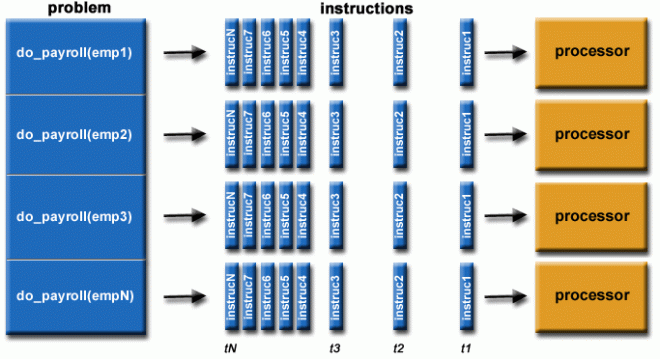
\includegraphics[width=0.5\textwidth]{parallelProblem2.png}
  \end{center}
  \vfill
  {\tiny https://hpc.llnl.gov/documentation/tutorials/introduction-parallel-computing-tutorial}
\end{frame}
%------------------------------------------------------------------------------
\begin{frame}
  \frametitle{Concorrência vs Paralelismo}
  \vspace{-4mm}
  \begin{itemize}
    \item \textbf{Concorrência} - múltiplas tarefas estão logicamente ativas ao mesmo tempo.
    \item \textbf{Paralelismo} - múltiplas tarefas estão realmente ativas ao mesmo tempo.
  \end{itemize}
  \begin{center}
	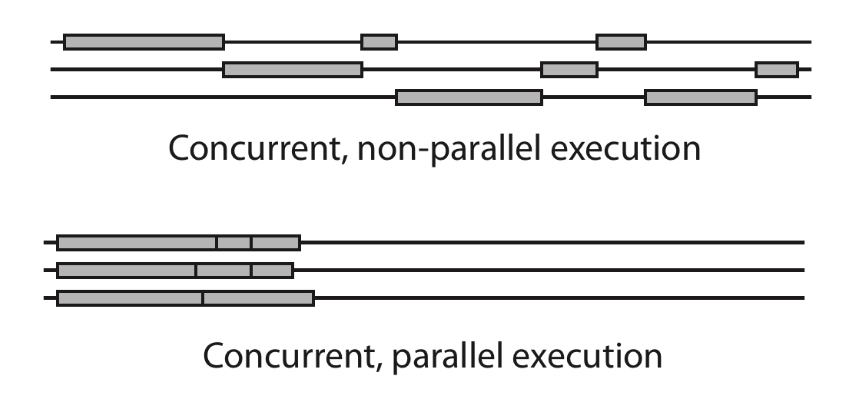
\includegraphics[width=0.7\textwidth]{concorrente1.png}
  \end{center}
  %{\footnotesize \url{https://www.karlrupp.net/2018/02/42-years-of-microprocessor-trend-data/}}
\end{frame}
%------------------------------------------------------------------------------
\begin{frame}
  \frametitle{Concorrência vs Paralelismo}
  \vspace{-4mm}
  \begin{itemize}
    \item \textbf{Concorrência} - múltiplas tarefas estão logicamente ativas ao mesmo tempo.
    \item \textbf{Paralelismo} - múltiplas tarefas estão realmente ativas ao mesmo tempo.
  \end{itemize}
  \begin{center}
	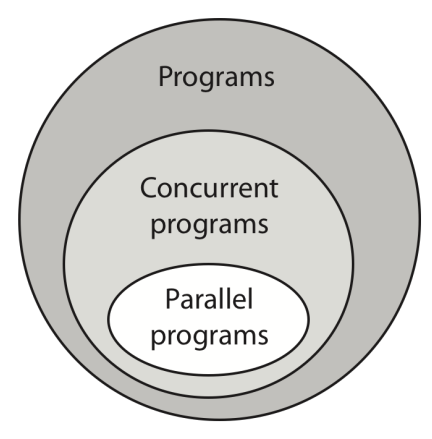
\includegraphics[width=0.3\textwidth]{concorrente2.png}
  \end{center}
  %{\footnotesize \url{https://www.karlrupp.net/2018/02/42-years-of-microprocessor-trend-data/}}
\end{frame}
%%%%%%%%%%%%%%%%%%%%%%%%%%%%%%%%%%%%%%%%%%%%%%%%%%%%%%%%%%%%%%%%%%%%%%%%%%%%%%
\section{Metodologia PCAM}
%%%%%%%%%%%%%%%%%%%%%%%%%%%%%%%%%%%%%%%%%%%%%%%%%%%%%%%%%%%%%%%%%%%%%%%%%%%%%%%
\begin{frame}
  \frametitle{Metodologia PCAM}
  \vspace{-3mm}
   \begin{columns}
     \begin{column}{0.6\textwidth}
      \begin{itemize}
        \item Descrito por Ian Foster no livro \emph{Designing and Building Parallel Programs}.
        \item Metodologia com quatro estágios.
          \begin{itemize}
            \item Particionamento
            \item Comunicação
            \item Aglomeração
            \item Mapeamento
          \end{itemize}
      \end{itemize}
     \end{column}
     \begin{column}{0.4\textwidth}
        \begin{center}
        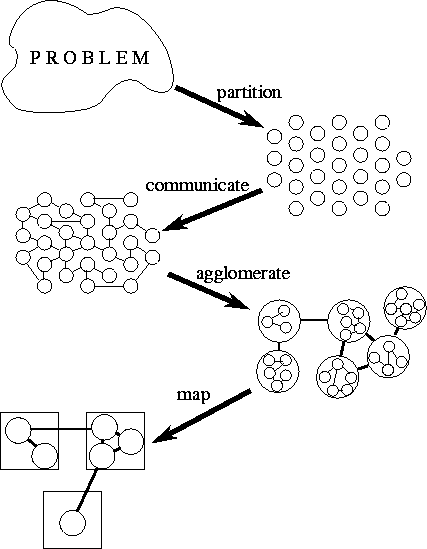
\includegraphics[width=\textwidth]{pcam.png}
        \end{center}
     \end{column}
   \end{columns}
  {\tiny https://www.mcs.anl.gov/~itf/dbpp/}
\end{frame}
%------------------------------------------------------------------------------
%%%%%%%%%%%%%%%%%%%%%%%%%%%%%%%%%%%%%%%%%%%%%%%%%%%%%%%%%%%%%%%%%%%%%%%%%%%%%%
\subsection{Particionamento}
%%%%%%%%%%%%%%%%%%%%%%%%%%%%%%%%%%%%%%%%%%%%%%%%%%%%%%%%%%%%%%%%%%%%%%%%%%%%%%%
\begin{frame}
  \frametitle{Particionamento}
  \vspace{-2mm}
  \begin{itemize}
    \item Identificar o máximo de oportunidade de paralelismo
    \item Decompor o problema em dados e/ou operações
    \item Definimos a \emph{granularidade}
      \begin{itemize}
        \item Tamanho da tarefa gerada
        \item Grão fino, ou grão grosso
      \end{itemize}
    \item Checklist:
      \begin{itemize}
        \item O número de tarefas é maior que o de processadores?
        \item O tamanho das tarefas é 
        \item O número de tarefas escala com o tamanho?
        \item É possível particionar de outras formas?
      \end{itemize}
  \end{itemize}
  \vspace{-5mm}
   \begin{columns}
     \begin{column}{0.6\textwidth}
        \begin{center}
          \begin{figure}
        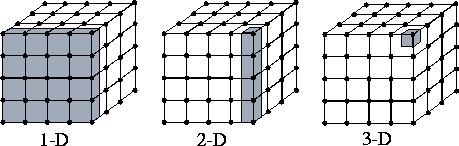
\includegraphics[width=0.8\textwidth]{cubos.png}
            \caption{Divisão por dados}
          \end{figure}
        \end{center}
     \end{column}
     \begin{column}{0.4\textwidth}
        \begin{center}
          \begin{figure}
        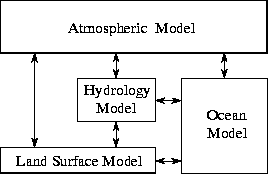
\includegraphics[width=0.8\textwidth]{functional.png}
            \caption{Divisão funcional}
          \end{figure}
        \end{center}
     \end{column}
   \end{columns}
\end{frame}
%------------------------------------------------------------------------------
%%%%%%%%%%%%%%%%%%%%%%%%%%%%%%%%%%%%%%%%%%%%%%%%%%%%%%%%%%%%%%%%%%%%%%%%%%%%%%
\subsection{Comunicação}
%%%%%%%%%%%%%%%%%%%%%%%%%%%%%%%%%%%%%%%%%%%%%%%%%%%%%%%%%%%%%%%%%%%%%%%%%%%%%%%
\begin{frame}
  \frametitle{Comunicação}
  \vspace{-2mm}
  \begin{itemize}
    \item O particionamento gera tarefas que executam concorrentemente mas não idependentemente (em alguns casos)
    \item Comunicação deve satisfazer dependências
    \item Depende da arquitetura/plataforma 
    \item Checklist:
      \begin{itemize}
        \item As comunicações são uniformes?
        \item A comunicação é para poucos vizinhos?
        \item As comunicações podem ser concorrentes?
        \item Podemos mesclar comunicação com processamento?
      \end{itemize}
  \end{itemize}
  \vspace{-5mm}
   \begin{columns}
     \begin{column}{0.6\textwidth}
        \begin{flushright}
          \begin{figure}
        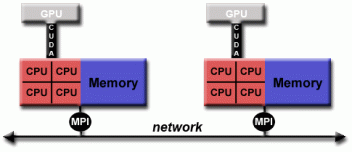
\includegraphics[width=0.8\textwidth]{hybrid_model2.png}
            \caption{Comunicação}
          \end{figure}
        \end{flushright}
     \end{column}
     \begin{column}{0.4\textwidth}
        \begin{flushleft}
          \begin{figure}
        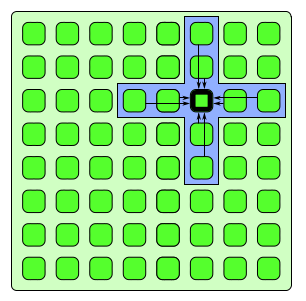
\includegraphics[width=0.4\textwidth]{stencil.png}
            \caption{Stencil}
          \end{figure}
        \end{flushleft}
     \end{column}
   \end{columns}
\end{frame}
%%%%%%%%%%%%%%%%%%%%%%%%%%%%%%%%%%%%%%%%%%%%%%%%%%%%%%%%%%%%%%%%%%%%%%%%%%%%%%
\subsection{Aglomeração}
%%%%%%%%%%%%%%%%%%%%%%%%%%%%%%%%%%%%%%%%%%%%%%%%%%%%%%%%%%%%%%%%%%%%%%%%%%%%%%%
\begin{frame}
  \frametitle{Aglomeração}
  \vspace{-2mm}
   \begin{columns}
     \begin{column}{0.6\textwidth}
      \begin{itemize}
        \item As tarefas criadas são pequenas? Eficientes?
        \item Na aglomeração, revisamos o particionamento e comunicação
        \item Um grande número de tarefas pequenas não produz um algoritmo paralelo eficiente
        \item Evitamos que o tempo de comunicação domine a computação
          \begin{itemize}
            \item Deve-se assumir que comunicações geram sobrecusto considerável.
          \end{itemize}
        \item Uma das técnicas é replicar/duplicar o processamento para reduzir comunicação.
          \begin{itemize}
            \item \emph{Ghost zones}
          \end{itemize}
      \end{itemize}
     \end{column}
     \begin{column}{0.4\textwidth}
        \begin{center}
          \begin{figure}
        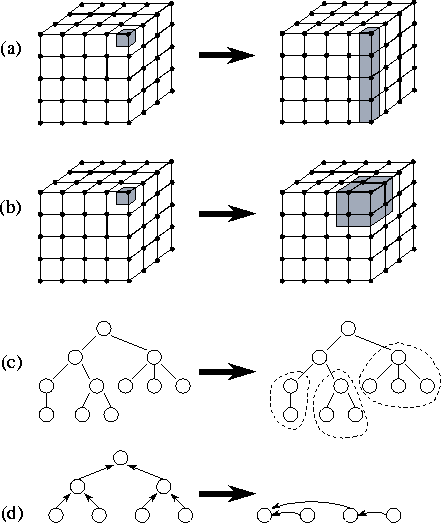
\includegraphics[width=\textwidth]{aglomeracao.png}
            \caption{Stencil}
          \end{figure}
        \end{center}
     \end{column}
   \end{columns}
\end{frame}
%------------------------------------------------------------------------------
\begin{frame}
  \frametitle{Aglomeração}
  \vspace{-2mm}
   \begin{columns}
     \begin{column}{0.6\textwidth}
      \begin{itemize}
        \item Checklist:
          \begin{itemize}
            \item Aglomeração reduz comunicações e aumenta localidade?
            \item Replicar/duplicar tem custo benefício?
            \item Agrupar deixa o grão homogeneo?
            \item As tarefas escalam?
            \item Sobrecusto do código paralelo com relação ao sequencial?
          \end{itemize}
      \end{itemize}
     \end{column}
     \begin{column}{0.4\textwidth}
        \begin{center}
          \begin{figure}
        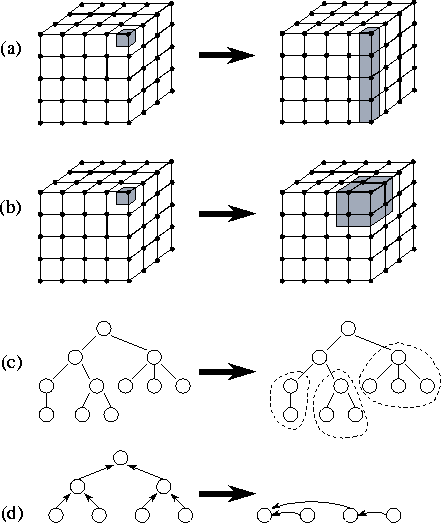
\includegraphics[width=\textwidth]{aglomeracao.png}
            \caption{Stencil}
          \end{figure}
        \end{center}
     \end{column}
   \end{columns}
\end{frame}
%%%%%%%%%%%%%%%%%%%%%%%%%%%%%%%%%%%%%%%%%%%%%%%%%%%%%%%%%%%%%%%%%%%%%%%%%%%%%%
\subsection{Mapeamento}
%%%%%%%%%%%%%%%%%%%%%%%%%%%%%%%%%%%%%%%%%%%%%%%%%%%%%%%%%%%%%%%%%%%%%%%%%%%%%%%
\begin{frame}
  \frametitle{Mapeamento}
  \vspace{-2mm}
   \begin{columns}
     \begin{column}{0.6\textwidth}
      \begin{itemize}
        \item Mapear tarefas para processador
        \item Objetivos:
          \begin{itemize}
            \item Colocar tarefas concorrentes em diferentes processadores
            \item Colocar tarefa que comunicam no mesmo processador (localidade)
          \end{itemize}
        \item O mapeamento é \textsc{NP-completo}
        \item Decomposicão fixa é trivial, outros casos nem tanto
          \begin{itemize}
            \item Estático 
            \item Dinâmico
          \end{itemize}
      \item Esta etapa também é conhecida por \emph{balanceamento de carga}
          \begin{itemize}
            \item Realizado pelo \emph{escalonador de tarefas}
          \end{itemize}
      \end{itemize}
     \end{column}
     \begin{column}{0.4\textwidth}
        \begin{center}
        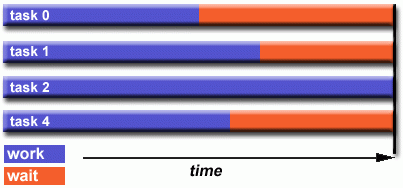
\includegraphics[width=\textwidth]{load_bal1.png}
        \end{center}
     \end{column}
   \end{columns}
\end{frame}
%------------------------------------------------------------------------------
\begin{frame}
  \frametitle{Mapeamento}
  \vspace{-4mm}
  \begin{center}
	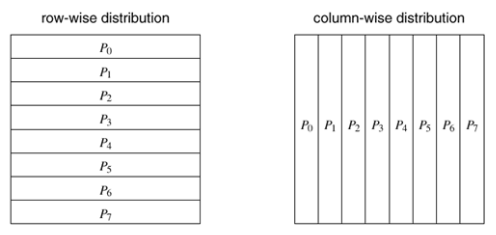
\includegraphics[width=0.8\textwidth]{map1.png}
  \end{center}
  \vfill
  {\tiny Introduction to Parallel Computing, Grama et al, 2003.}
\end{frame}
%------------------------------------------------------------------------------
\begin{frame}
  \frametitle{Mapeamento}
  \vspace{-4mm}
  \begin{center}
	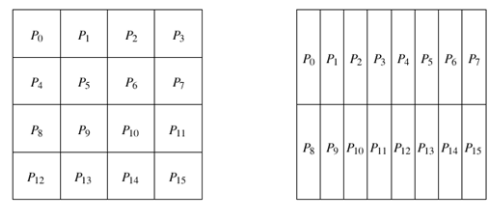
\includegraphics[width=0.8\textwidth]{map2.png}
  \end{center}
  \vfill
  {\tiny Introduction to Parallel Computing, Grama et al, 2003.}
\end{frame}
%------------------------------------------------------------------------------
\begin{frame}
  \frametitle{Mapeamento}
  \vspace{-4mm}
  \begin{center}
	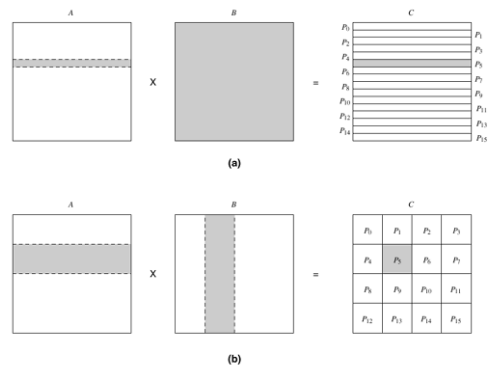
\includegraphics[width=0.6\textwidth]{map3.png}
  \end{center}
  \vfill
  {\tiny Introduction to Parallel Computing, Grama et al, 2003.}
\end{frame}
%------------------------------------------------------------------------------
\begin{frame}
  \frametitle{Mapeamento}
  \vspace{-4mm}
  \begin{center}
	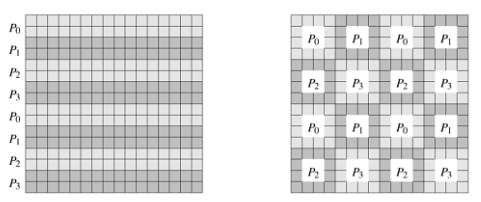
\includegraphics[width=0.8\textwidth]{map4.png}
  \end{center}
  \vfill
  {\tiny Introduction to Parallel Computing, Grama et al, 2003.}
\end{frame}
%------------------------------------------------------------------------------
\begin{frame}
  \frametitle{Mapeamento}
  \vspace{-4mm}
  \begin{center}
	
\includegraphics[width=0.8\textwidth]{map5.png}
  \end{center}
  \vfill
  {\tiny Introduction to Parallel Computing, Grama et al, 2003.}
\end{frame}
%------------------------------------------------------------------------------
\begin{frame}
  \frametitle{Mapeamento}
  \vspace{-4mm}
  \begin{center}
	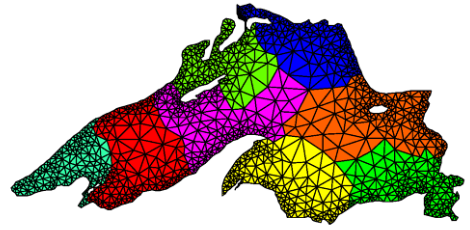
\includegraphics[width=0.8\textwidth]{map6.png}
  \end{center}
  \vfill
  {\tiny Introduction to Parallel Computing, Grama et al, 2003.}
\end{frame}
%------------------------------------------------------------------------------
\begin{frame}
  \frametitle{Mapeamento}
  \vspace{-4mm}
  \begin{center}
	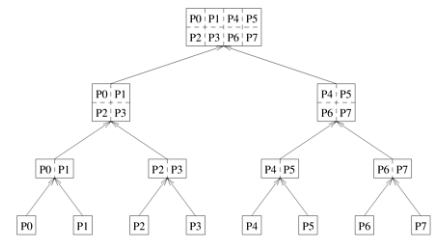
\includegraphics[width=0.8\textwidth]{map7.png}
  \end{center}
  \vfill
  {\tiny Introduction to Parallel Computing, Grama et al, 2003.}
\end{frame}
%------------------------------------------------------------------------------
\begin{frame}
  \frametitle{Mapeamento}
  \vspace{-4mm}
  \begin{center}
	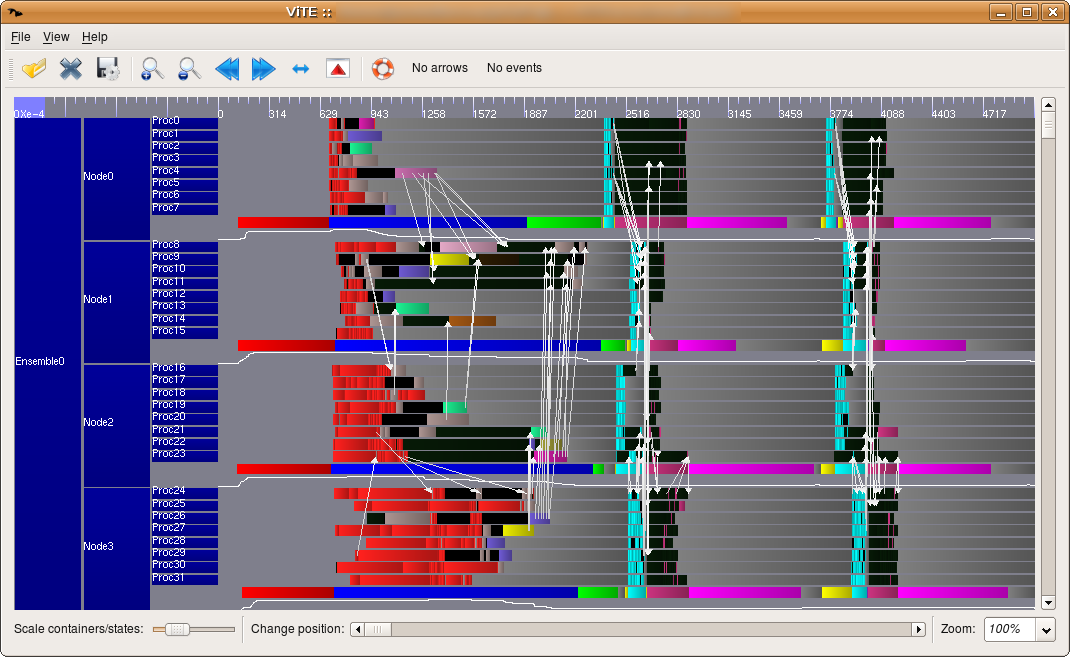
\includegraphics[width=0.8\textwidth]{vite.png}
  \end{center}
  \vfill
  {\tiny https://solverstack.gitlabpages.inria.fr/vite/}
\end{frame}
%------------------------------------------------------------------------------
%-- %%%%%%%%%%%%%%%%%%%%%%%%%%%%%%%%%%%%%%%%%%%%%%%%%%%%%%%%%%%%%%%%%%%%%%%%%%%%%%
%-- \section{Taxonomia de Flynn}
%-- %%%%%%%%%%%%%%%%%%%%%%%%%%%%%%%%%%%%%%%%%%%%%%%%%%%%%%%%%%%%%%%%%%%%%%%%%%%%%%%
%-- \begin{frame}
%--   \frametitle{Taxonomia de Flynn}
%--   \vspace{-4mm}
%--   \begin{center}
%-- 	\includegraphics[width=0.7\textwidth]{flynn.png}
%--   \end{center}
%--   {\footnotesize Stallings, W. Computer Organization and Architecture. 2017.}
%-- \end{frame}
%-- %------------------------------------------------------------------------------
%-- \begin{frame}
%--   \frametitle{Single instruction, single data (SISD)}
%--     \begin{itemize}
%--         \item Uma instrução opera sobre um dado de cada vez.
%--         \item Arquitetura Von Neumann.
%--     \end{itemize}
%-- 	%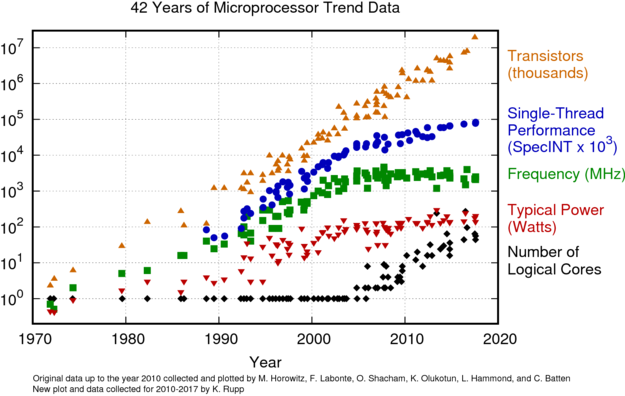
\includegraphics[width=0.7\textwidth]{42-years-processor-trend-625x396.png}
%-- \end{frame}
%-- %------------------------------------------------------------------------------
%-- \begin{frame}
%--   \frametitle{Single instruction, multiple data (SIMD)}
%--     \begin{itemize}
%--       \item O processador executa um conjunto de operações \textbf{simultaneamente} sobre múltiplos dados (matrizes ou vetores)
%--       \item Muito usada em HPC
%--       \item Exemplos de arquiteturas
%--       \begin{itemize}
%--           \item NEC SX-Aurora TSUBASA
%--           \item GPUs como Single Instruction Multiple Threads (SIMT)
%--       \end{itemize}
%--     \end{itemize}
%-- \end{frame}
%-- %------------------------------------------------------------------------------
%-- \begin{frame}
%--   \frametitle{NEC SX-Aurora TSUBASA}
%--   \vspace{-3mm}
%--       \begin{itemize}
%--           \item Cada Vector Engine Processor pode ter até 16x cores.
%--           \item FMA - Fused multiply-add \texttt{a*b + c}
%--       \end{itemize}
%--   \begin{center}
%-- 	\includegraphics[width=0.9\textwidth]{Vectorpipes.png}
%--   \end{center}
%--   {\footnotesize \url{https://www.nec.com/en/global/solutions/hpc/sx/architecture.html}}
%-- \end{frame}
%-- %------------------------------------------------------------------------------
%-- \begin{frame}
%--   \frametitle{Graphics Processing Unit (GPU)}
%--   %\vspace{-3mm}
%--       \begin{itemize}
%--           \item CPUs executam uma sequência de instruções o mais rápido possível
%--           \item GPUs executam um grande número de instruções concorrentes 
%--       \end{itemize}
%--   \begin{center}
%-- 	\includegraphics[width=0.8\textwidth]{gpus.png}
%--   \end{center}
%--   \vspace{-4mm}
%--   {\footnotesize \url{https://docs.nvidia.com/cuda/cuda-c-programming-guide/}}
%-- \end{frame}
%-- %------------------------------------------------------------------------------
%-- \begin{frame}
%--   \frametitle{Graphics Processing Unit (GPU)}
%--   \vspace{-5mm}
%--   \begin{center}
%-- 	\includegraphics[width=0.7\textwidth]{memory-hierarchy.png}
%--   \end{center}
%--   \vspace{-4mm}
%--   {\footnotesize \url{https://docs.nvidia.com/cuda/cuda-c-programming-guide/}}
%-- \end{frame}
%-- %------------------------------------------------------------------------------
%-- \begin{frame}
%--   \frametitle{Graphics Processing Unit (GPU)}
%--   \vspace{-4mm}
%--   \begin{center}
%-- 	\includegraphics[width=0.7\textwidth]{cuda-sms.png}
%--   \end{center}
%--   \vspace{-4mm}
%--   {\footnotesize https://developer.nvidia.com/blog/cuda-refresher-cuda-programming-model/}
%-- \end{frame}
%-- %------------------------------------------------------------------------------
%-- \begin{frame}
%--   \frametitle{Graphics Processing Unit (GPU)}
%--   \vspace{-4mm}
%--   \begin{center}
%-- 	\includegraphics[width=0.7\textwidth]{memory-hierarchy-in-gpus-2.png}
%--   \end{center}
%--   \vspace{-4mm}
%--   {\footnotesize https://developer.nvidia.com/blog/cuda-refresher-cuda-programming-model/}
%-- \end{frame}
%-- %------------------------------------------------------------------------------
%-- %\begin{frame}
%-- %  \frametitle{História do C++}
%-- %    \begin{columns}
%-- %      \begin{column}{0.7\textwidth}
%-- %     \end{column}
%-- %      \begin{column}{0.3\textwidth}
%-- %      \end{column}
%-- %    \end{columns}
%-- %\end{frame}
%-- %------------------------------------------------------------------------------
%-- % TODO: excessao, etc
%-- %\begin{frame}
%-- %  \frametitle{Entrada e saída}
%-- %  \begin{itemize}
%-- %  \item 
%-- %  \end{itemize}
%-- %\end{frame}
%-- %------------------------------------------------------------------------------
%-- %\begin{frame}
%-- %  \frametitle{Entrada e saída}
%-- %  \begin{itemize}
%-- %  \item 
%-- %  \end{itemize}
%-- %\end{frame}
%-- %------------------------------------------------------------------------------
%-- \begin{frame}
%--   \frametitle{Multiple instruction, single data (MISD)}
%--     \begin{itemize}
%--         \item Múltiplas instruções operam sobre um dado de cada vez.
%--         \item Nunca desenvolvida
%--         \item Algumas vezes associado a \emph{systolic arrays}
%--     \end{itemize}
%-- 	%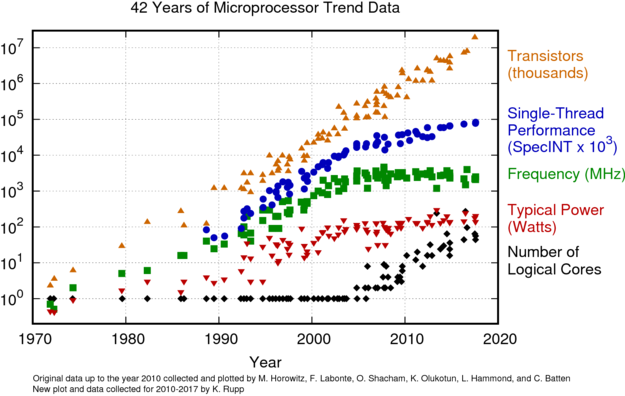
\includegraphics[width=0.7\textwidth]{42-years-processor-trend-625x396.png}
%-- \end{frame}
%-- %------------------------------------------------------------------------------
%-- \begin{frame}
%--   \frametitle{Multiple instruction, multiple data (MIMD)}
%--     \begin{itemize}
%--         \item Múltiplas instruções operam sobre múltiplos dados simultaneamento.
%--         \item Memória compartilhada
%--             \begin{itemize}
%--               \item Multiprocessador simétrico (SMP)
%--               \item Sistemas com acesso não-uniforme a memória (NUMA)
%--               \item Processadores multicore
%--             \end{itemize}
%--     \end{itemize}
%-- 	%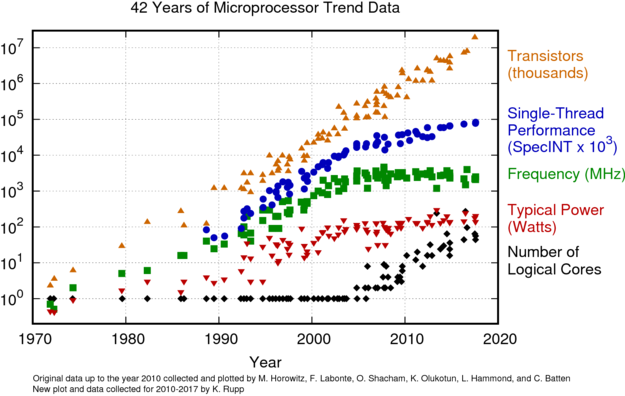
\includegraphics[width=0.7\textwidth]{42-years-processor-trend-625x396.png}
%-- \end{frame}
%-- %------------------------------------------------------------------------------
%-- \begin{frame}
%--   \frametitle{IBM Cell processor}
%--     \begin{itemize}
%--         \item Processador multi-core baseado no PowerPC
%--         \item 1x IBM PowerPC processing element (PPE)
%--         \item 8x  synergistic processing elements (SPE)
%--         \item A movimentação de dados entre caches dependia do programador
%--     \end{itemize}
%--   \vspace{-3mm}
%--   \begin{center}
%-- 	\includegraphics[width=0.6\textwidth]{cell1.png}
%--   \end{center}
%-- 	%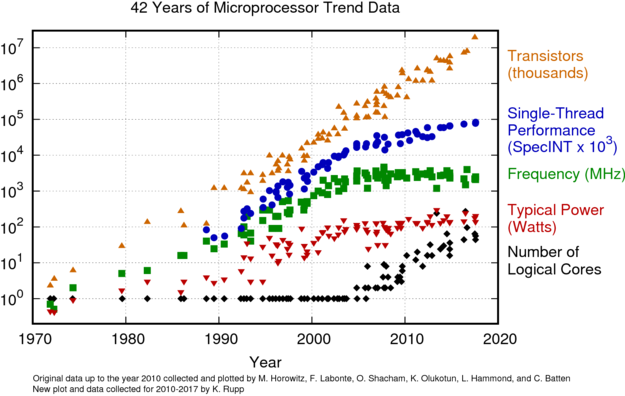
\includegraphics[width=0.7\textwidth]{42-years-processor-trend-625x396.png}
%-- \end{frame}
%-- %------------------------------------------------------------------------------
%-- \begin{frame}
%--   \frametitle{US Condor Cluster (PS3)}
%--   \vspace{-3mm}
%--   \begin{center}
%-- 	\includegraphics[width=0.8\textwidth]{condor.jpg}
%--   \end{center}
%-- \end{frame}
%-- %------------------------------------------------------------------------------
%-- \begin{frame}
%--   \frametitle{Intel Knights Landing}
%--     \begin{columns}
%--       \begin{column}{0.4\textwidth}
%--     \begin{itemize}
%--         \item Processador manycore x86
%--         \item 68 núcleos, totalizando 272 núcleos e 1088 threads, 1.4 GHz
%--         \item 96 GB DDR4 RAM + 16 GB HBM MCDRAM
%--         \item Sistema Linux próprio com comandos 
%--     \end{itemize}
%--      \end{column}
%--       \begin{column}{0.6\textwidth}
%--         \begin{center}
%--         \includegraphics[width=0.9\textwidth]{knl1.png}
%--         \end{center}
%--       \end{column}
%--     \end{columns}
%-- 	%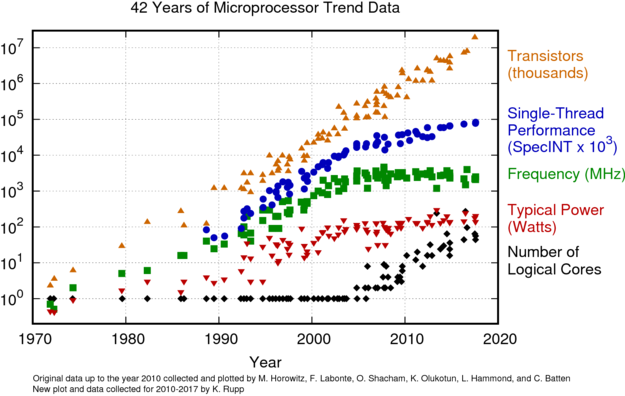
\includegraphics[width=0.7\textwidth]{42-years-processor-trend-625x396.png}
%-- \end{frame}
%-- %------------------------------------------------------------------------------
%-- \begin{frame}
%--   \frametitle{Intel Knights Landing}
%--   \vspace{-3mm}
%--   \begin{center}
%-- 	\includegraphics[width=0.9\textwidth]{knl2.png}
%--   \end{center}
%-- \end{frame}
%-- %------------------------------------------------------------------------------
%-- \begin{frame}
%--   \frametitle{Intel Knights Landing}
%--   \vspace{-3mm}
%--   \begin{center}
%-- 	\includegraphics[width=0.9\textwidth]{knl-flat-mcdram.png}
%--   \end{center}
%-- \end{frame}
%-- %------------------------------------------------------------------------------
%-- \begin{frame}
%--   \frametitle{Sun UltraSPARC T2}
%--   \vspace{-3mm}
%--   \begin{center}
%--     \includegraphics[width=0.5\textwidth]{UltraSPARC-T2.png}
%--   \end{center}
%-- \end{frame}
%-- %------------------------------------------------------------------------------
%-- \begin{frame}
%--   \frametitle{ARM big.LITTLE}
%--   \vspace{-3mm}
%--   \begin{center}
%--     \includegraphics[width=0.9\textwidth]{biglittle.png}
%--   \end{center}
%-- \end{frame}
%-- %------------------------------------------------------------------------------
%-- %% {\setbeamercolor{background canvas}{bg=}
%-- %% \includepdf[pages=52-64,%
%-- %%     %pagecommand={\begin{frame}[default]{}\end{frame}},
%-- %%     pagecommand={},
%-- %% %    #4,%
%-- %% turn=false,noautoscale=false,column=false,columnstrict=false,openright=false,frame=false]{palestra-pet-si-jun2015.pdf}%
%-- %% }
%%%%%%%%%%%%%%%%%%%%%%%%%%%%%%%%%%%%%%%%%%%%%%%%%%%%%%%%%%%%%%%%%%%%%%%%%%%%%%
\section{Conclusão PCAM}
%%%%%%%%%%%%%%%%%%%%%%%%%%%%%%%%%%%%%%%%%%%%%%%%%%%%%%%%%%%%%%%%%%%%%%%%%%%%%%%
%------------------------------------------------------------------------------
\begin{frame}
  \frametitle{Conclusão PCAM}
  \vspace{-3mm}
   \begin{columns}
     \begin{column}{0.6\textwidth}
      \begin{itemize}
        \item Primeiro particionamos o problema em pequenos pedaços
        \begin{itemize}
          \item Dados ou funcional
        \end{itemize}
        \item Organizamos a comunicação entre tarefas quando necessário
        \item Analisamos a aglomeração para reduzir comunicação e sobrecusto paralelo
        \item Por fim, mapeamos tarefas para processadores.
        \begin{itemize}
          \item Estático, balanceamento de carga, ou escalonamento
        \end{itemize}
      \end{itemize}
     \end{column}
     \begin{column}{0.4\textwidth}
        \begin{center}
        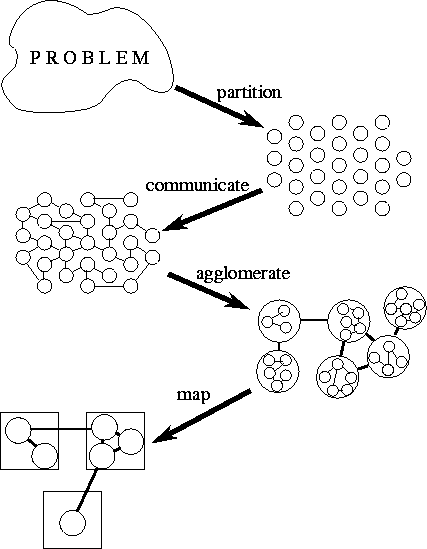
\includegraphics[width=\textwidth]{pcam.png}
        \end{center}
     \end{column}
   \end{columns}
  {\tiny https://www.mcs.anl.gov/~itf/dbpp/}
\end{frame}
%------------------------------------------------------------------------------
\begin{frame}[plain]{}
  \begin{center}
    \vspace{2cm}
    \Large{https://joao-ufsm.github.io/par2023a/}
    
    \vspace{1cm}
    
\includegraphics[width=2cm]{logo_ufsm}
    \hspace{0.5cm}
    
\includegraphics[width=2cm]{logo_inf}
  \end{center}
\end{frame}
%------------------------------------------------------------------------------

\end{document}
